%
\section{Implementation}\label{sec:implementation}
This chapter explains how the component is developed. The ways to overcome the design challenges, some of the findings during the development have been written down.
%
\subsection{System Characteristics}
When beginning the implementation, I decided to use a simple yet powerful programming language for both frontend and backend applications to obtain my results. The programming languages which I selected was javascript for the frontend and C\# for the backend. I used the Visual Studio Code IDE for the frontend and Visual Studio 2019 for the backend to simplify my programming work. The configuration of the computer used for implementation is as follows:

{\bf Operating System:} Windows 10 Enterprise 2016 - 64-bit\\
{\bf Processor:} Intel Core i7-6700 @ 3.4GHz\\
{\bf RAM:} 16GB\\
{\bf HDD:} 500GB\\


The software support tools used for frontend implementation are listed as follows:

{\bf Programming Language:} Javascript\\
{\bf IDE:} Visual Studio Code\\
{\bf Packet Manager:} npm\\
{\bf Version Control:} Azure Repos\\


The software support tools used for backend implementation are listed as follows:

{\bf Programming Language:} C\#\\
{\bf IDE:} Visual Studio 2019\\
{\bf Packet Manager:} NuGet\\
{\bf Database:} Azure Data Storage - Containers\\
{\bf Version Control:} Azure Repos\\


All the infrastructure and software that I used are provided by evosoft GmbH.
\subsection{OSS Component Analyzer}
The \acs{OSS} component analyzer is a starting point in the process of scanning the \acs{OSS} components from a project. It is a front-end module, and it is implemented in the Angular framework using typescript language. The GUI interface of this module requires four inputs from the user: the project name, description, members, and project source directory. It has two essential tasks before it proceeds to the evaluation process. In the first task, the module should find the required configuration file in the project. This configuration file identification was made with the help of a dependency manager. Each application framework has its dependency manager, and it generates a unique configuration file for the application framework. The table ~\ref{tab:configFiles} shows all the config files of each application framework. The \acs{OSS} component names and versions will be listed in the config files.
\begin{table}[h!]
\begin{center}
 \begin{tabular}{ |c|c|c|c| } 
 	\hline
 	Application Framework & Dependency Manager & Config file & File Type \\
 	\hline
 	.NET(Console Application) & Nuget & .csproj file & XML \\ 
 	Angular Framework & npm & package.json & JSON \\ 
 	Microsoft TFS & Nuget & app.config & XML \\ 
 	Django & npm & requirremen.txt & Text\\ 
 	Ruby on Rails & Rubygem & gemfile & File \\ 
 	Laravel & composer & composer.json & JSON \\ 
 	Gradle projects & gradle & build.gradle & GRADLE \\ 
 	Maven projects & POM & pom.xml & XML \\ 
 	.NET & Nuget & packages.config & XML \\ 
 	\hline
 \end{tabular}
\caption{Configuration file of each application framework.}\label{tab:configFiles}
\end{center} 
\end{table}

Once the respective config is identified from the project, the targeted data should be scrapped from config files. To achieve this, automated scrapping methods are used based on the config file type. For instance, the user is scanning the Maven project, and then according to the table, the config file is an XML file, so, therefore, to scrap the targeted data \acs{DOM} parsing method is used. Likewise, for \acs{JSON} file, JSON parsing methods can be used, text pattern matching methods can be used for a text file, Gemfile, FIle and GRADLE files. After scrapping the targeted data, the next task is to generate a JSON object with the general project information and scrapped \ac{OSS} information and will be ready to send it to the \acs{OSS} evaluation process. 

The figure ~\ref{fig:Analyzer_Activity_Diagram} will illustrate the technical flow of how the \acs{OSS} component is extracted from the software project and send the meta-information like component name and version for the evaluation process. Firstly, the user must give the public input such as project name, project description, project members and the complete source code directory. Once the data is submitted, the first validation stage is to check whether the required config file is available in the directory to identify the project's application framework. Once the scanner identifies the application framework, the \acs{OSS} components will be extracted based on the config file's file type. For instance, the scanner will search for the build if the user submits a Gradle project for scanning .gradle file, which looks like the figure ~\ref{fig:gradle} and will start the extraction process. In the extraction process, the build.gradle file is iterated and read line by line with the help of FileReader class in Angular framework until the line begins with a string "compile". The dependencies section is where all the project dependencies, which is the \acs{OSS} components, are registered, and we know that every dependency under the dependency section starts with the string "compile". So whenever the strings start with the string "compile", that particular line will consist of the component name and version. Then the component name and version will be extracted out by using text pattern matching functions. Likewise, the same type of extraction is performed for Django and Ruby on Rails projects. For the other projects, simple \acs{DOM} parser methods are used to extract the components because their file types are JSON and XML. Finally, the extracted components will be converted to a JSON object and the general information and sent to the backend application for the evaluation process.   

 \begin{figure}[H]
	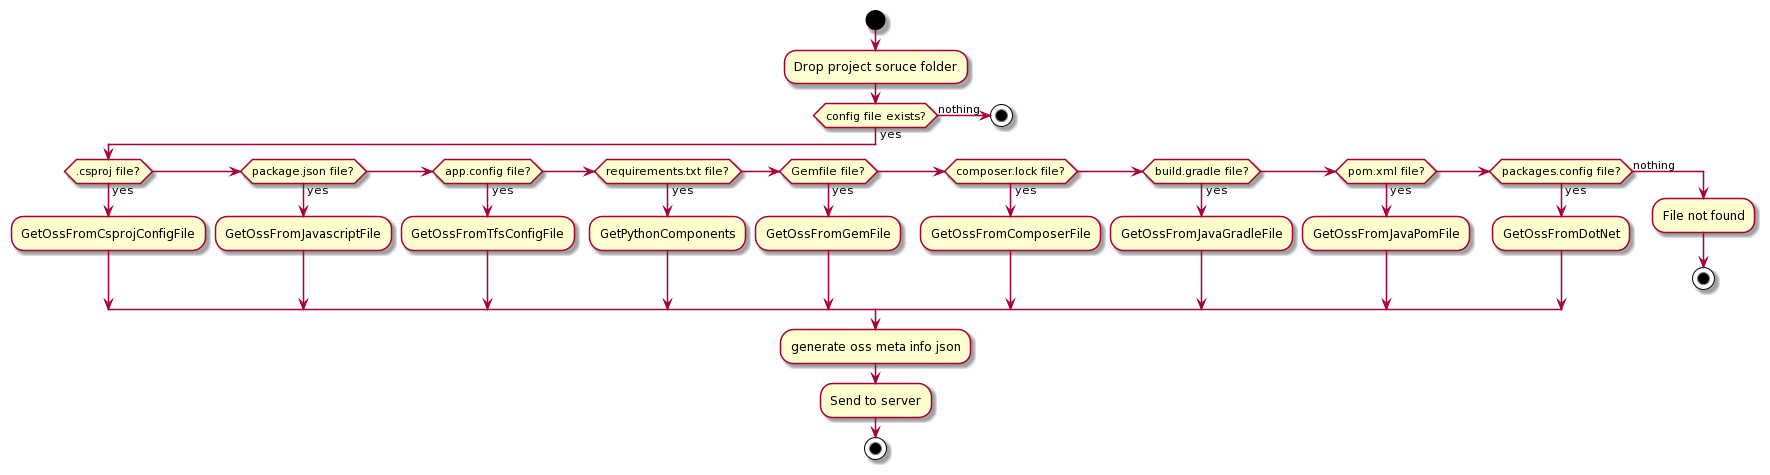
\includegraphics[width=15cm]{includes/OSS_Analyzer_Activity_Diagram.png}
	\centering
	\caption{\acs{OSS} Component Analyzer Activity Diagram}
	\label{fig:Analyzer_Activity_Diagram}
\end{figure}
\subsection{Component Evaluator}
The \acs{OSS} component evaluator is the final process of finding the vulnerabilities with the help of a vulnerability database. This backend application is developed by using ASP.NET. The searching can be done with the help of \acs{NVD}'s API services \cite{NVDApi}. Once the backend application receives the JSON objects from the client application, the application will start searching the OSS components in the \acs{NVD} database by using the endpoints provided in the API documentation \cite{NVDApi}. First component names and versions will be searched under the \acs{CPE} dictionary to verify the product has been registered in the \acs{CPE}. If the component is found in the \acs{CPE} dictionary, the service returns all the results of the component name. To verify the component name and the version is not a normal process because the \acs{CPE} name has its naming specification. The figure ~\ref{fig:cpe_name} is an example of the \acs{CPE} naming specification.
 \begin{figure}[h!]
	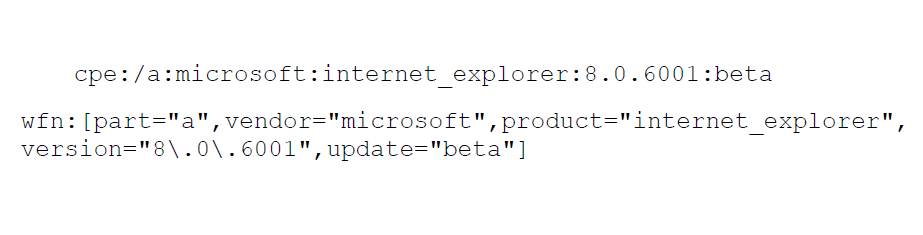
\includegraphics[width=15cm]{includes/cpe_name.png}
	\centering
	\caption{CPE name specification}
	\label{fig:cpe_name}
\end{figure}
From the figure ~\ref{fig:cpe_name} it is visible that the component name and version are in the 3rd and fourth position of the \acs{CPE} string. The given component name and version must be verified with the \acs{CPE} name. As the second stage of verification, the given component name and \acs{CPE} name is verified again by using the Levenshtein distance algorithm. Having this second stage of verification can make sure the component does not have any spelling mistakes. Once the \acs{CPE} name is validated with the given component, the next step will be retrieving the \acs{CVE} details using the \acs{CPE} name to find out the vulnerability information. \acs{CVE} retrieval API services are used to find the vulnerability information \cite{NVDApi}. 

The figure ~\ref{fig:Evaluator_Activity_Diagram} will illustrate the technical side of how the \acs{OSS} components are evaluated with the help of the NVD database. Firstly, the backend application will receive the request sent from the client application, and the OSS components in the JSON object will be iterated to evaluate each component. In the iteration, the first process is to search the component name in the CPE dictionary to verify the component is registered in the CPE dictionary by using the "https://services.nvd.nist.gov/rest/json/cpes/1.0?keyword=" API endpoint. The results from the CPE dictionary will be iterated to find the exact component name of its version. The component name and version will be matched with the CPE name that looks like in the figure ~\ref{fig:cpe_name}. We already know that the vendor, product name and version are separated using the ":" character. In this case, first, the CPE name will be split using the ":" character and converted to an array. Now every 3rd and fourth position of the array will be matched with the given component name and version respectively for every iteration until finding the exact match. As the second stage of verification, the component name and the CPE product name will have a string distance evaluation using the Levenshtein distance algorithm to spellcheck. If the distance result is 0, it means the spelling match is perfect, but if the result is 1 to 2, still the component will be taken to the result, but it will be flagged as "recommended". If it is greater than or equal to 3, then the iteration will be skipped to the next component and flagged as "Not found". Once the OSS component name is verified against the CPE name, the next task is to search for the vulnerabilities in the CVE database by using the CPE name string. The vulnerabilities are searched using the "https://services.nvd.nist.gov/rest/json/cves/1.0?cpeMatchString=" API endpoint. The API endpoint requires cpeMatchString as an input parameter where we can give the CPE name as input and gives the vulnerability information of the particular CPE name like the figure ~\ref{fig:nvdOutput}. After collecting the vulnerability results of all the possible OSS components, the results will be converted as a JSON object. It will be saved in the Azure data storage as a blob container. 
\newpage 
\begin{figure}[h!]
	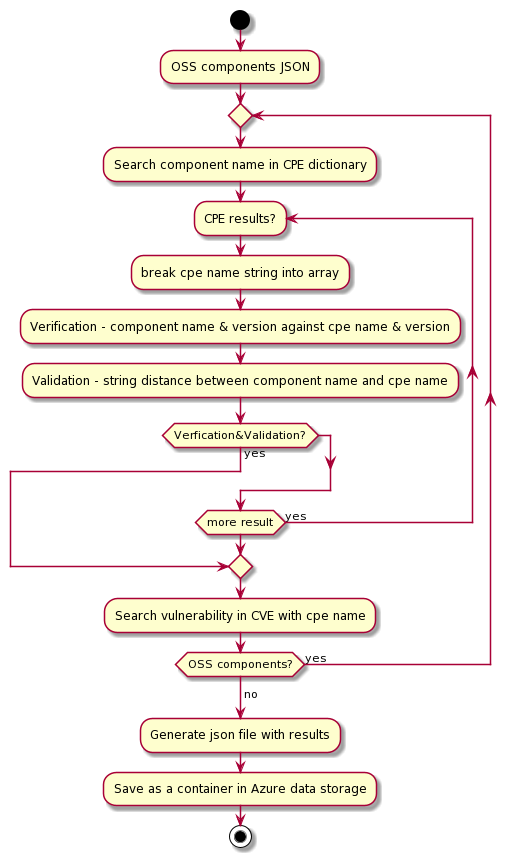
\includegraphics[width=15cm,height=20cm]{includes/OSS_Evaluator_Activity_Diagram.png}
	\centering
	\caption{\acs{OSS} Component Evaluator Activity Diagram}
	\label{fig:Evaluator_Activity_Diagram}
\end{figure} 
\newpage                                                                                      \newpage            
\subsection{Reporter}
The Reporter is the final module of the \acs{OSS} scanner, and it is implemented in the client-side of the application. This module is implemented in the Angular framework by using the jspdf library. The primary purpose of this module is to generate a report of the scanned projects by containing the \acs{CVSS} information of each \acs{OSS} component. The report will consist only of the necessary and human-understandable information in the report, so this makes the user have a clear understanding of the report and helps to make a decision. The information for the report will be retrieved from the Azure data storage.

The figure ~\ref{fig:Reporter_Activity_Diagram} shows the technical flow of how the report is downloaded. Once the user requests the backend application, the backend application will retrieve the blob container of the specific project which is requested. In the blob container, the JSON object is stored as blob data. Then the blob data is converted to a JSON object with relevant properties like both CVSS V2 and V3 data. Finally, with the help of the jspdf library, the results retrieved from the backend application is downloaded as a pdf file.  


%
\begin{figure}[h!]
	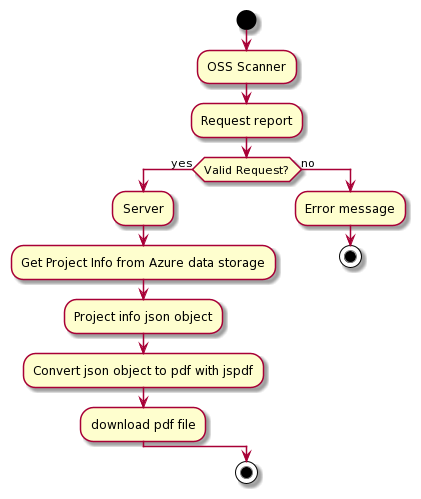
\includegraphics[width=10cm,height=15cm]{includes/Reporter_Activity_Diagram.png}
	\centering
	\caption{\acs{OSS} Component Evaluator Activity Diagram}
	\label{fig:Reporter_Activity_Diagram}
\end{figure}   